\documentclass[a4paper, amsfonts, amssymb, amsmath, reprint, showkeys, nofootinbib, twoside]{revtex4-1}
\usepackage[english]{babel}
\usepackage[utf8]{inputenc}
\usepackage[colorinlistoftodos, color=green!40, prependcaption]{todonotes}
\usepackage[pdftex, pdftitle={Article}, pdfauthor={Author}]{hyperref}
\usepackage{amsthm}
\usepackage{mathtools}
\usepackage{physics}
\usepackage{xcolor}
\usepackage{caption}
\usepackage{hyperref}
%\hypersetup{colorlinks=true, linkcolor=blue, urlcolor = blue}
\usepackage{amsmath}
\usepackage{amssymb}
\usepackage{graphicx}
\graphicspath{Images}
\usepackage[left=23mm,right=13mm,top=35mm,columnsep=15pt]{geometry} 
\usepackage{adjustbox}
\usepackage{placeins}
\usepackage[T1]{fontenc}
\usepackage{float}
%\usepackage{longtable}
\usepackage{csquotes}
\usepackage{refstyle}
\usepackage{lipsum}
\usepackage{booktabs}
\usepackage{upgreek}

\begin{document}

\title{Study of Polarisation of Light and Verification of Malus's Law}
\author{Swaroop Ramakant Avarsekar}
\email{swaroop.avarsekar@niser.ac.in}
\affiliation{School of Physical Sciences, National Institute of Science Education and Research, HBNI, Jatni -752050, India}
\date{\today}
	
\maketitle

\section{Introduction and Theory}
Polarisation is phenomenon where the oscillations of electric field of light is restricted to certain direction (axis). It is due to vibration of electron cloud around the atoms, resulting in certain plane. Unpolarised light is where the oscillations of electric field are rapid and random resulting in cancellation of effects. Unpolarised light can be polarised by restricting the electric field oscillations in one direction. Polariser having property of birefringent properties of crystals such as quartz, calcite etc, is used for such purpose. The incident unpolarised beam through polariser is transmitted with reduction of intensity by half. Analyser is identical to that of polariser. When analyser is placed after the polariser, the intensity of transmitted light from analyser varies with rotation of transmission axis as described by Malus's law.
\begin{equation}
	I=I_o.cos^2\theta
\end{equation}
Where $I$ is the intensity from analyser, $I_o$
 
\begin{figure}[H] %  figure placement: here, top, bottom, or page
	\centering
	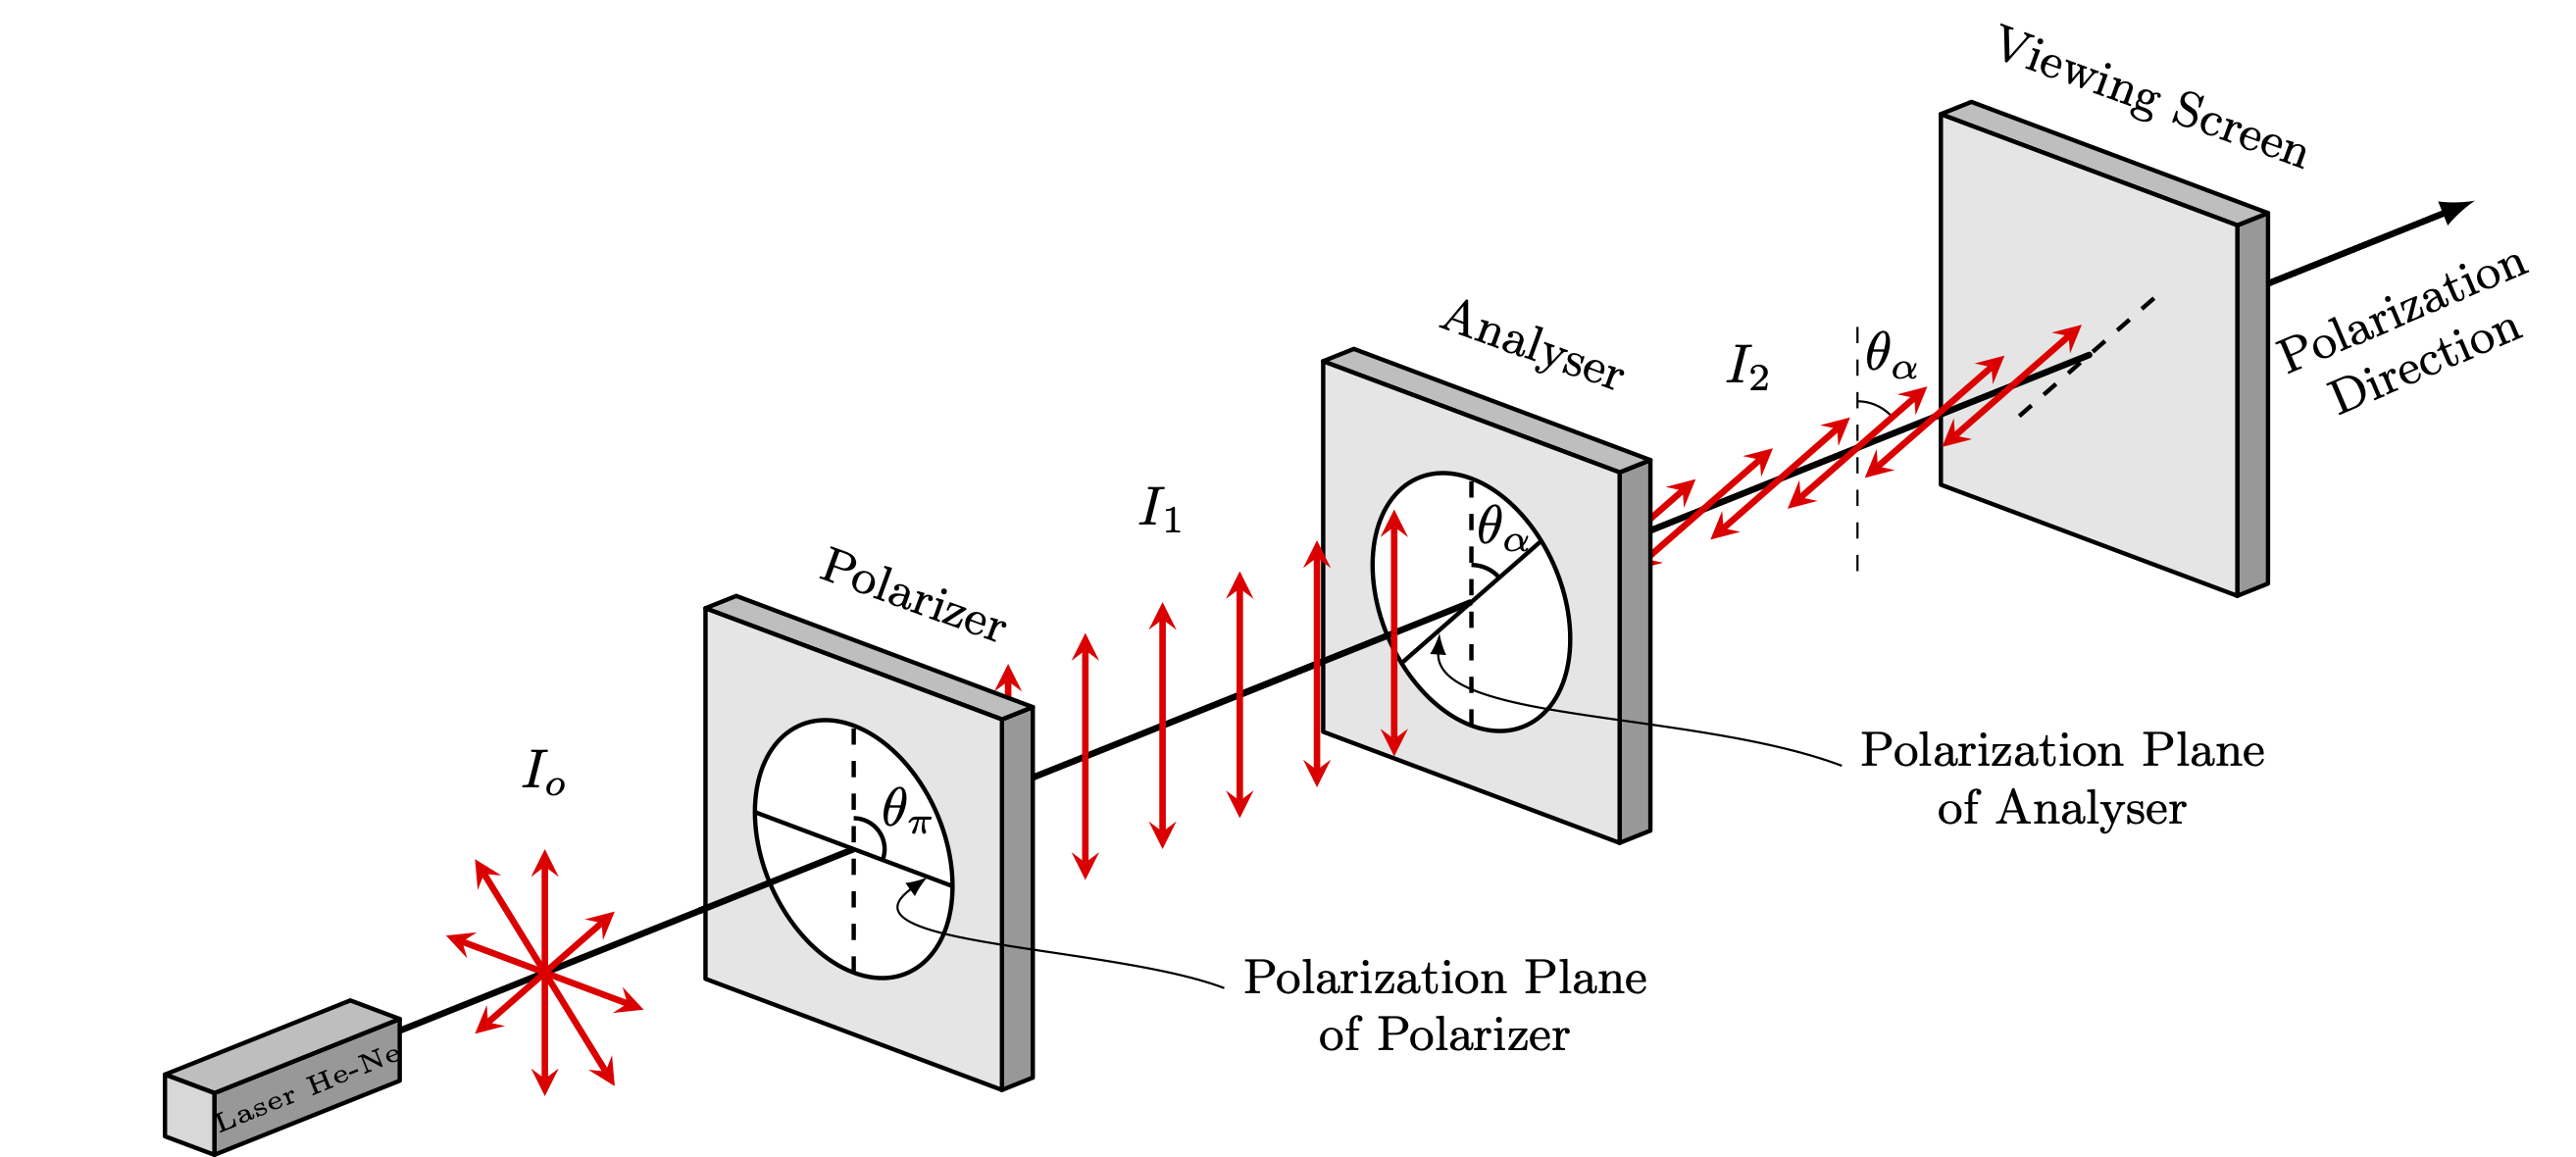
\includegraphics[width=8.3cm,height=4cm]{1} 
	\caption{Polariser and Analyser in working}
	\label{1}
\end{figure}

Waveplates, modify existing polarisations without attenuating, deviating or displacing the beams. They are also made of birefringent materials, where laser falling on those gets divided into two components, with ordinary (obey laws of refraction) ray , $n_o$ and extra ordinary ray (do not obey laws of refraction) $n_e$, causing relative phase difference between two emergent beams as,
\begin{equation}
	\upvarphi=2\pi(n_o-n_e)d/\lambda
\end{equation}
where d is thickness of crystal and $\lambda$ is wavelength of laser beam
 In half wave plate, the phase difference between two emergent beam is $\pi$ due to the thickness of the same.
 \begin{figure}[H] %  figure placement: here, top, bottom, or page
 	\centering
 	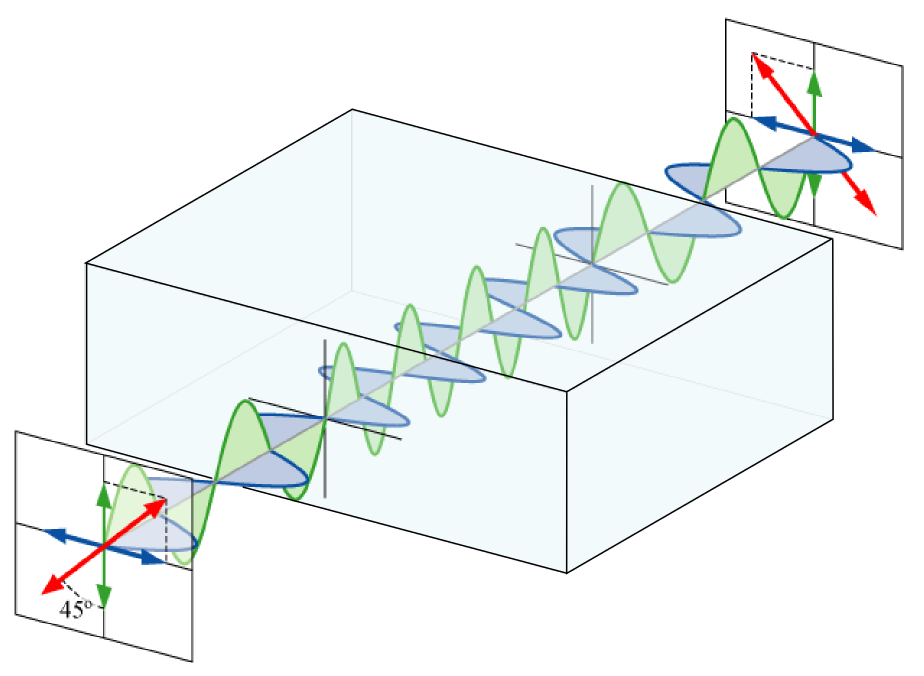
\includegraphics[width=8.3cm,height=4cm]{2} 
 	\caption{State of polarisation under half wave plate}
 	\label{2}
 \end{figure}

If the thickness is adjusted such that we get phase difference of $\pi/2$, then we obtain quarter wave plate. Normal incidence of linearly polarised light on half wave plate and plane of polarisation of HW plate is $45^{\circ}$ wrt fast axis, then emergent light will have circular polarisation, else elliptical polarisation.

 \begin{figure}[H] %  figure placement: here, top, bottom, or page
	\centering
	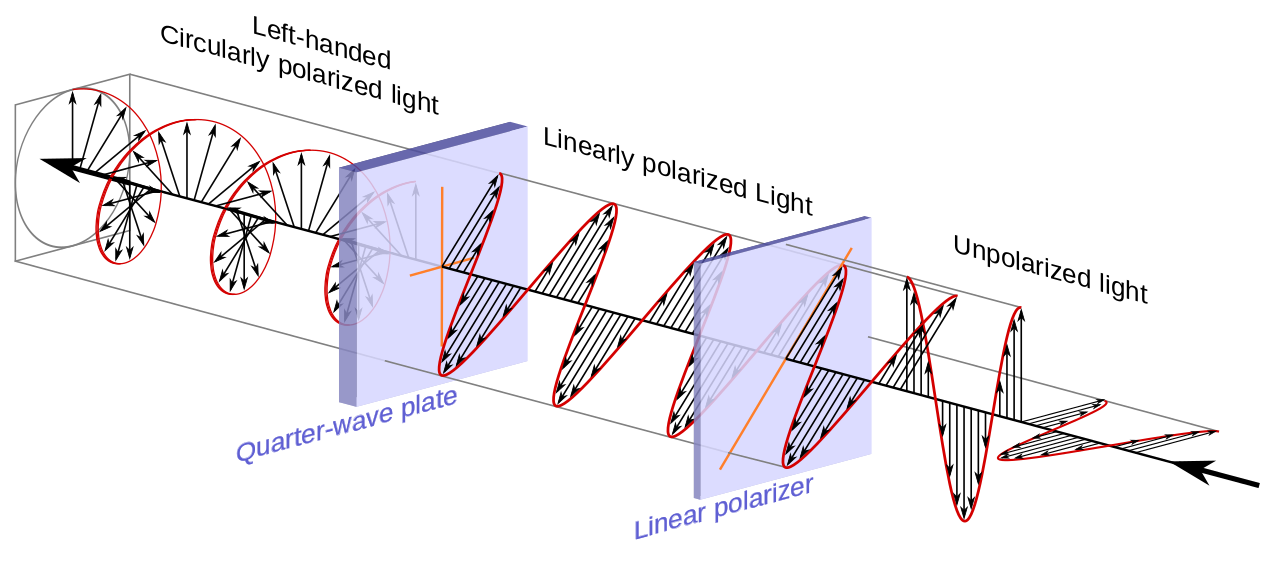
\includegraphics[width=8.3cm,height=4cm]{3} 
	\caption{State of polarisation under quarter wave plate}
	\label{3}
\end{figure}

\section{Experiment}
\subsection{Apparatus}
He-Ne Laser will be used to polarise, polariser along with analyser and half and quarter wave plates. A photodetector connected to multimeter is placed at other extreme to detect the current. Optical bench along with suitable post holders are also required.  
\subsection{Procedure}
Turn ON the laser for several minutes to achieve stable output. Align the polariser, laser and detector on the same axis. Measure the dark current (if there), on the multimeter by blocking laser from the detector. Rotate the polariser by $360^\circ$ to get two maxima. Inser the analyser between detector and polariser and adjust axis such that maximum current is obtained. Note down the angle, and rotate the analyser in steps of $10^\circ-20^\circ$, keeping polariser fixed to linearly polarise light and verify the Malus's law.

After $360^\circ$ rotation of the analyser, insert the half wave plate with axis set at zero, such that the axis is aligned. Note the angle. Rotate half wave plate to around $45^\circ$. Keeping the polariser unchanged, rotate the analyser till you observe two maxima and minima, note down the current reading. The polarisation is rotated by twice the angle of the half wave plate. To obtain the elliptical and circularly polarised light replace the half wave plate with quarter wave plate and align it with the same optical axis. Rotate the half wave plate to any angular position. To produce circularly polarised light, fix the position at $45^\circ$. Keeping polariser unchanged rotate the analyser till you observe two maxima and minima, note down the current values and plot it in polar projection. 

\begin{figure}[H] %  figure placement: here, top, bottom, or page
	\centering
	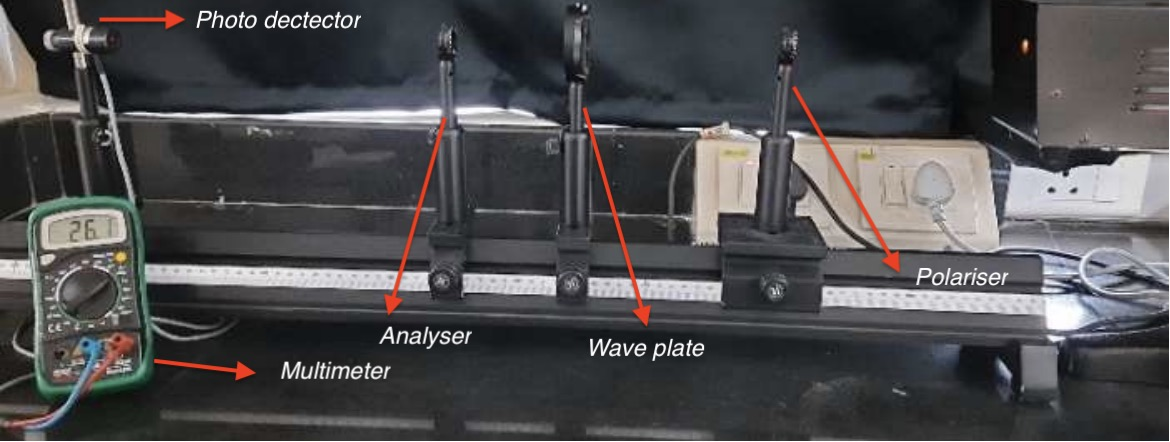
\includegraphics[width=8.3cm,height=5cm]{app} 
	\caption{Experimental setup in laboratory}
	\label{app}
\end{figure}

\subsection{Precautions}
\begin{enumerate}
\item{Block the Laser light from photo-detector when setting up the apparatus.}
\item{Perform experiment in dark room only and ensure there is no interference of unnecessary light.}
\item {Make sure to take the readings quickly as the detector heats up with long exposure of laser beam giving offset values.}
\end{enumerate}

\subsection{Observations}
\begin{figure}[H] %  figure placement: here, top, bottom, or page
	\centering
	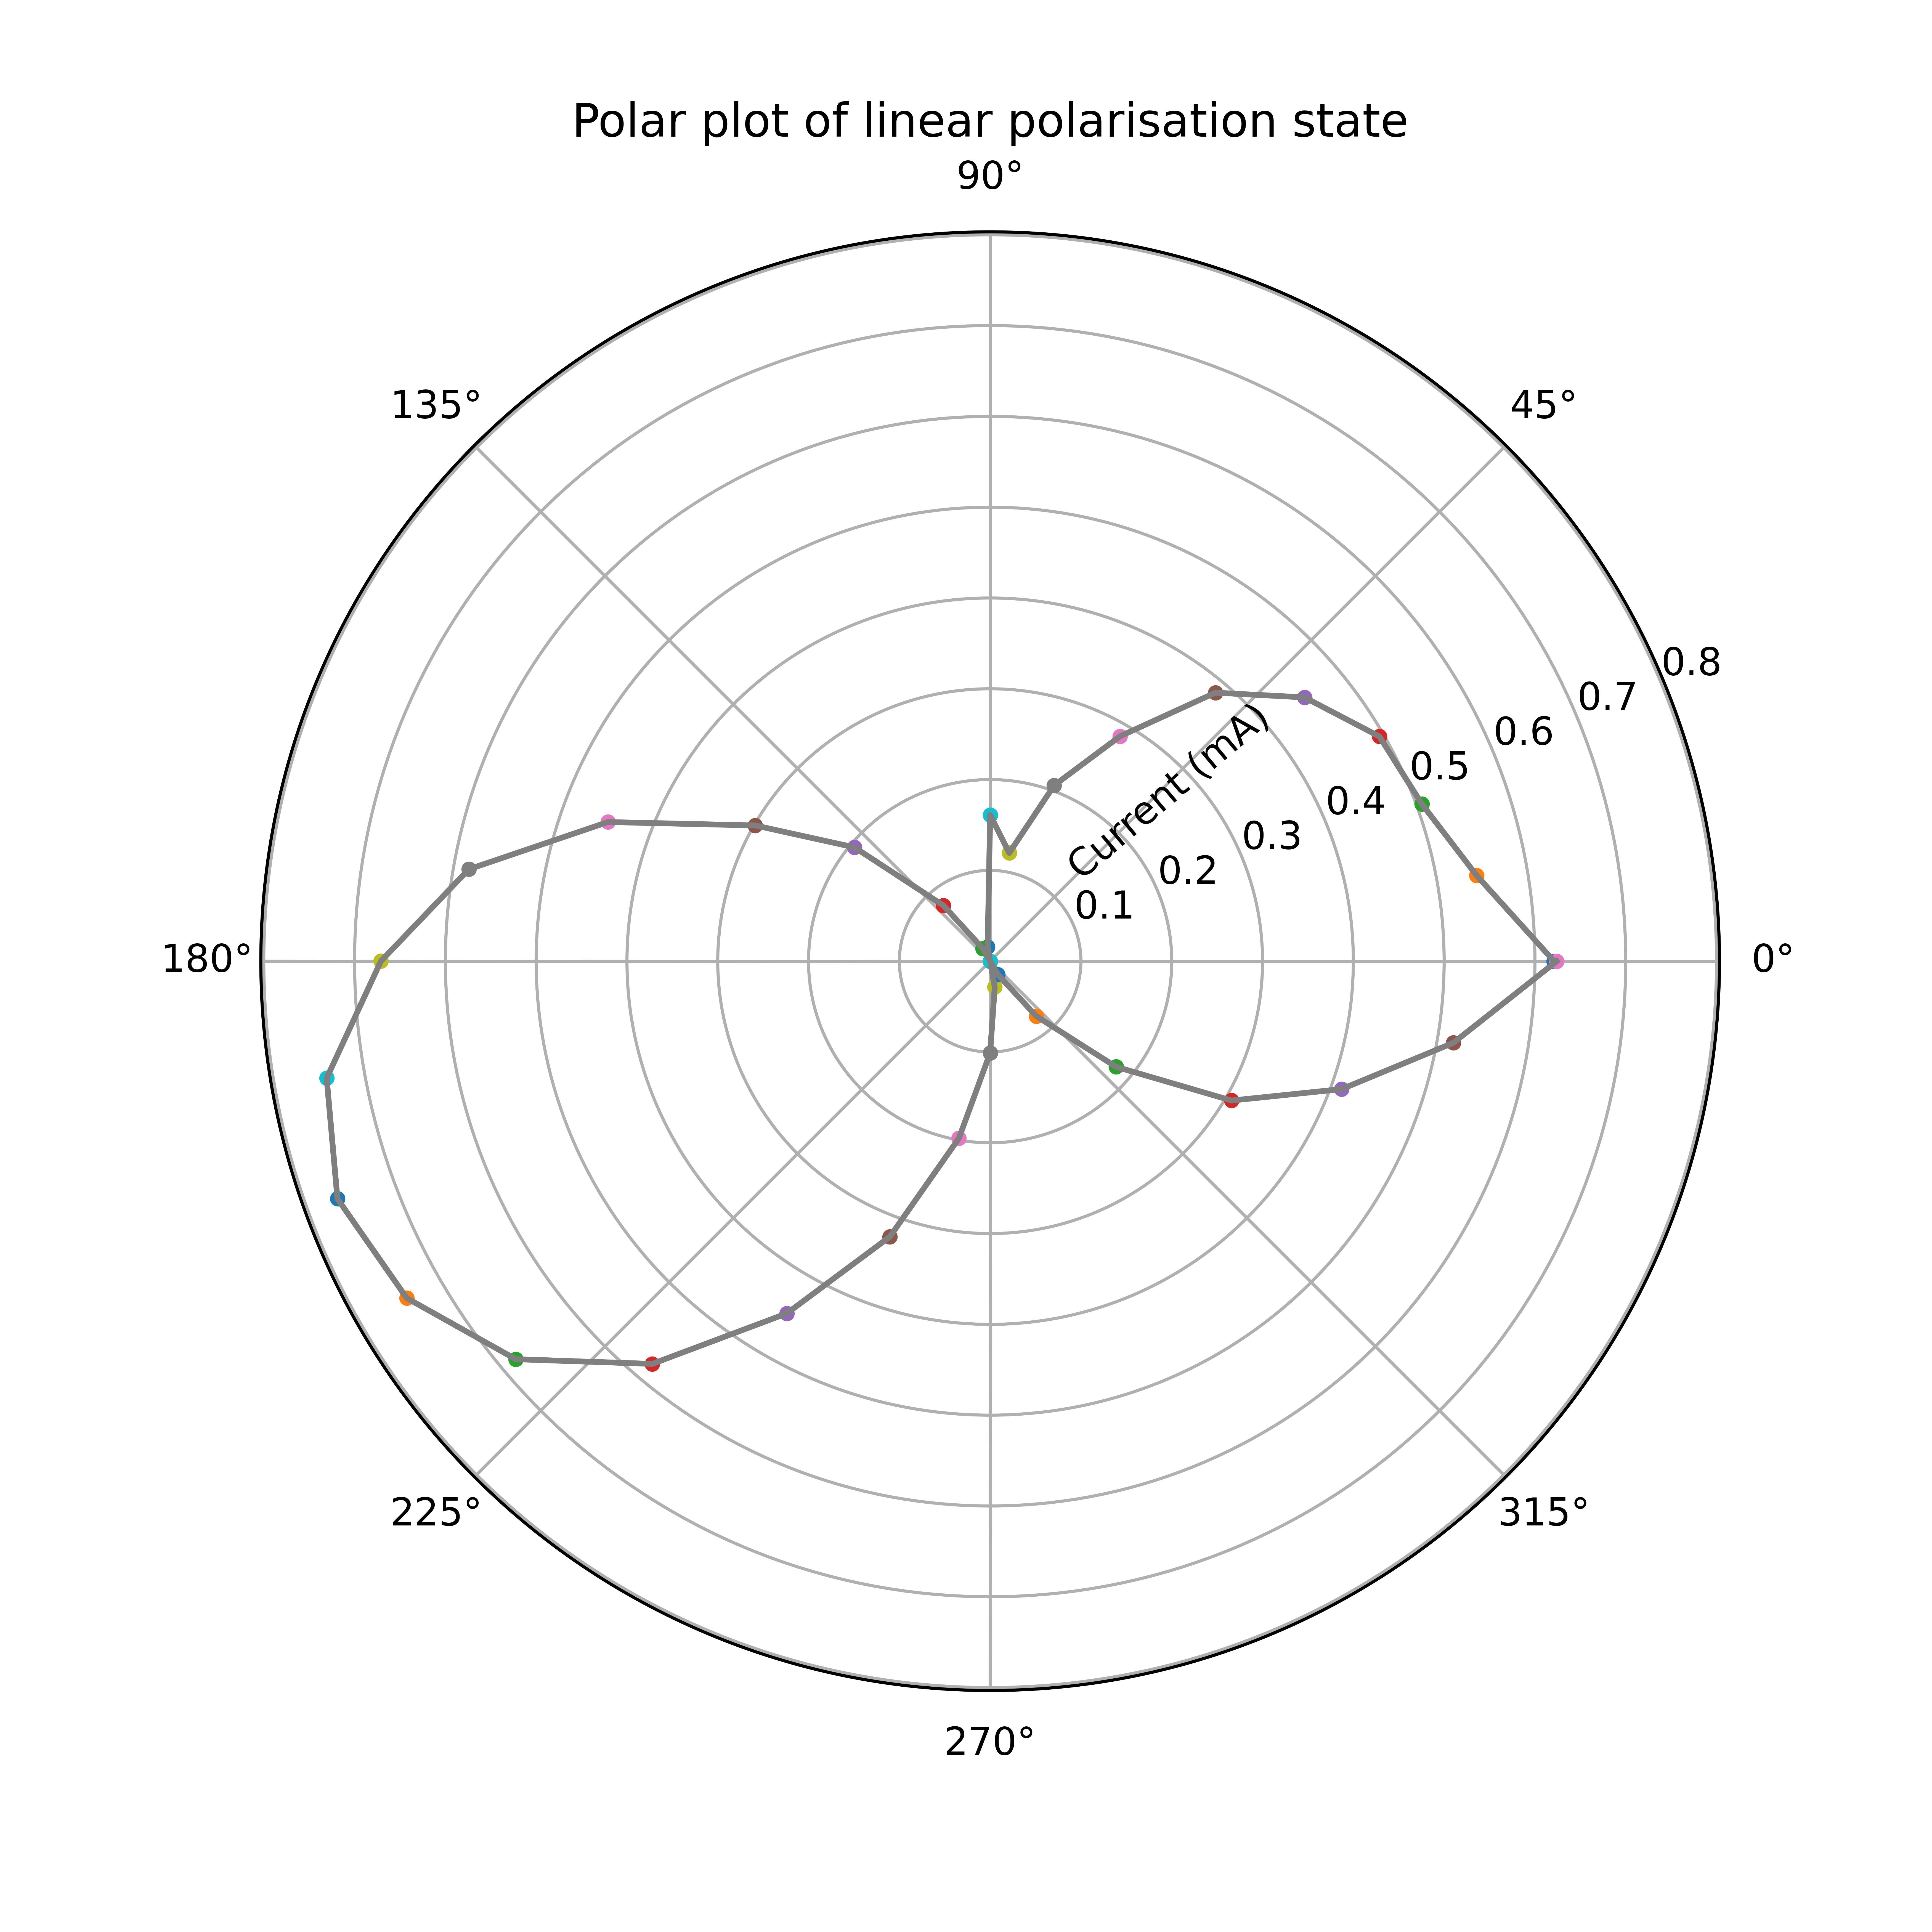
\includegraphics[width=8.3cm,height=8.3cm]{4} 
	\caption{Polar plot of linear polarisation of light where current is along the radial direction and angle is measured in analyser with respect to polariser.}
	\label{4}
\end{figure}

\begin{figure}[H] %  figure placement: here, top, bottom, or page
	\centering
	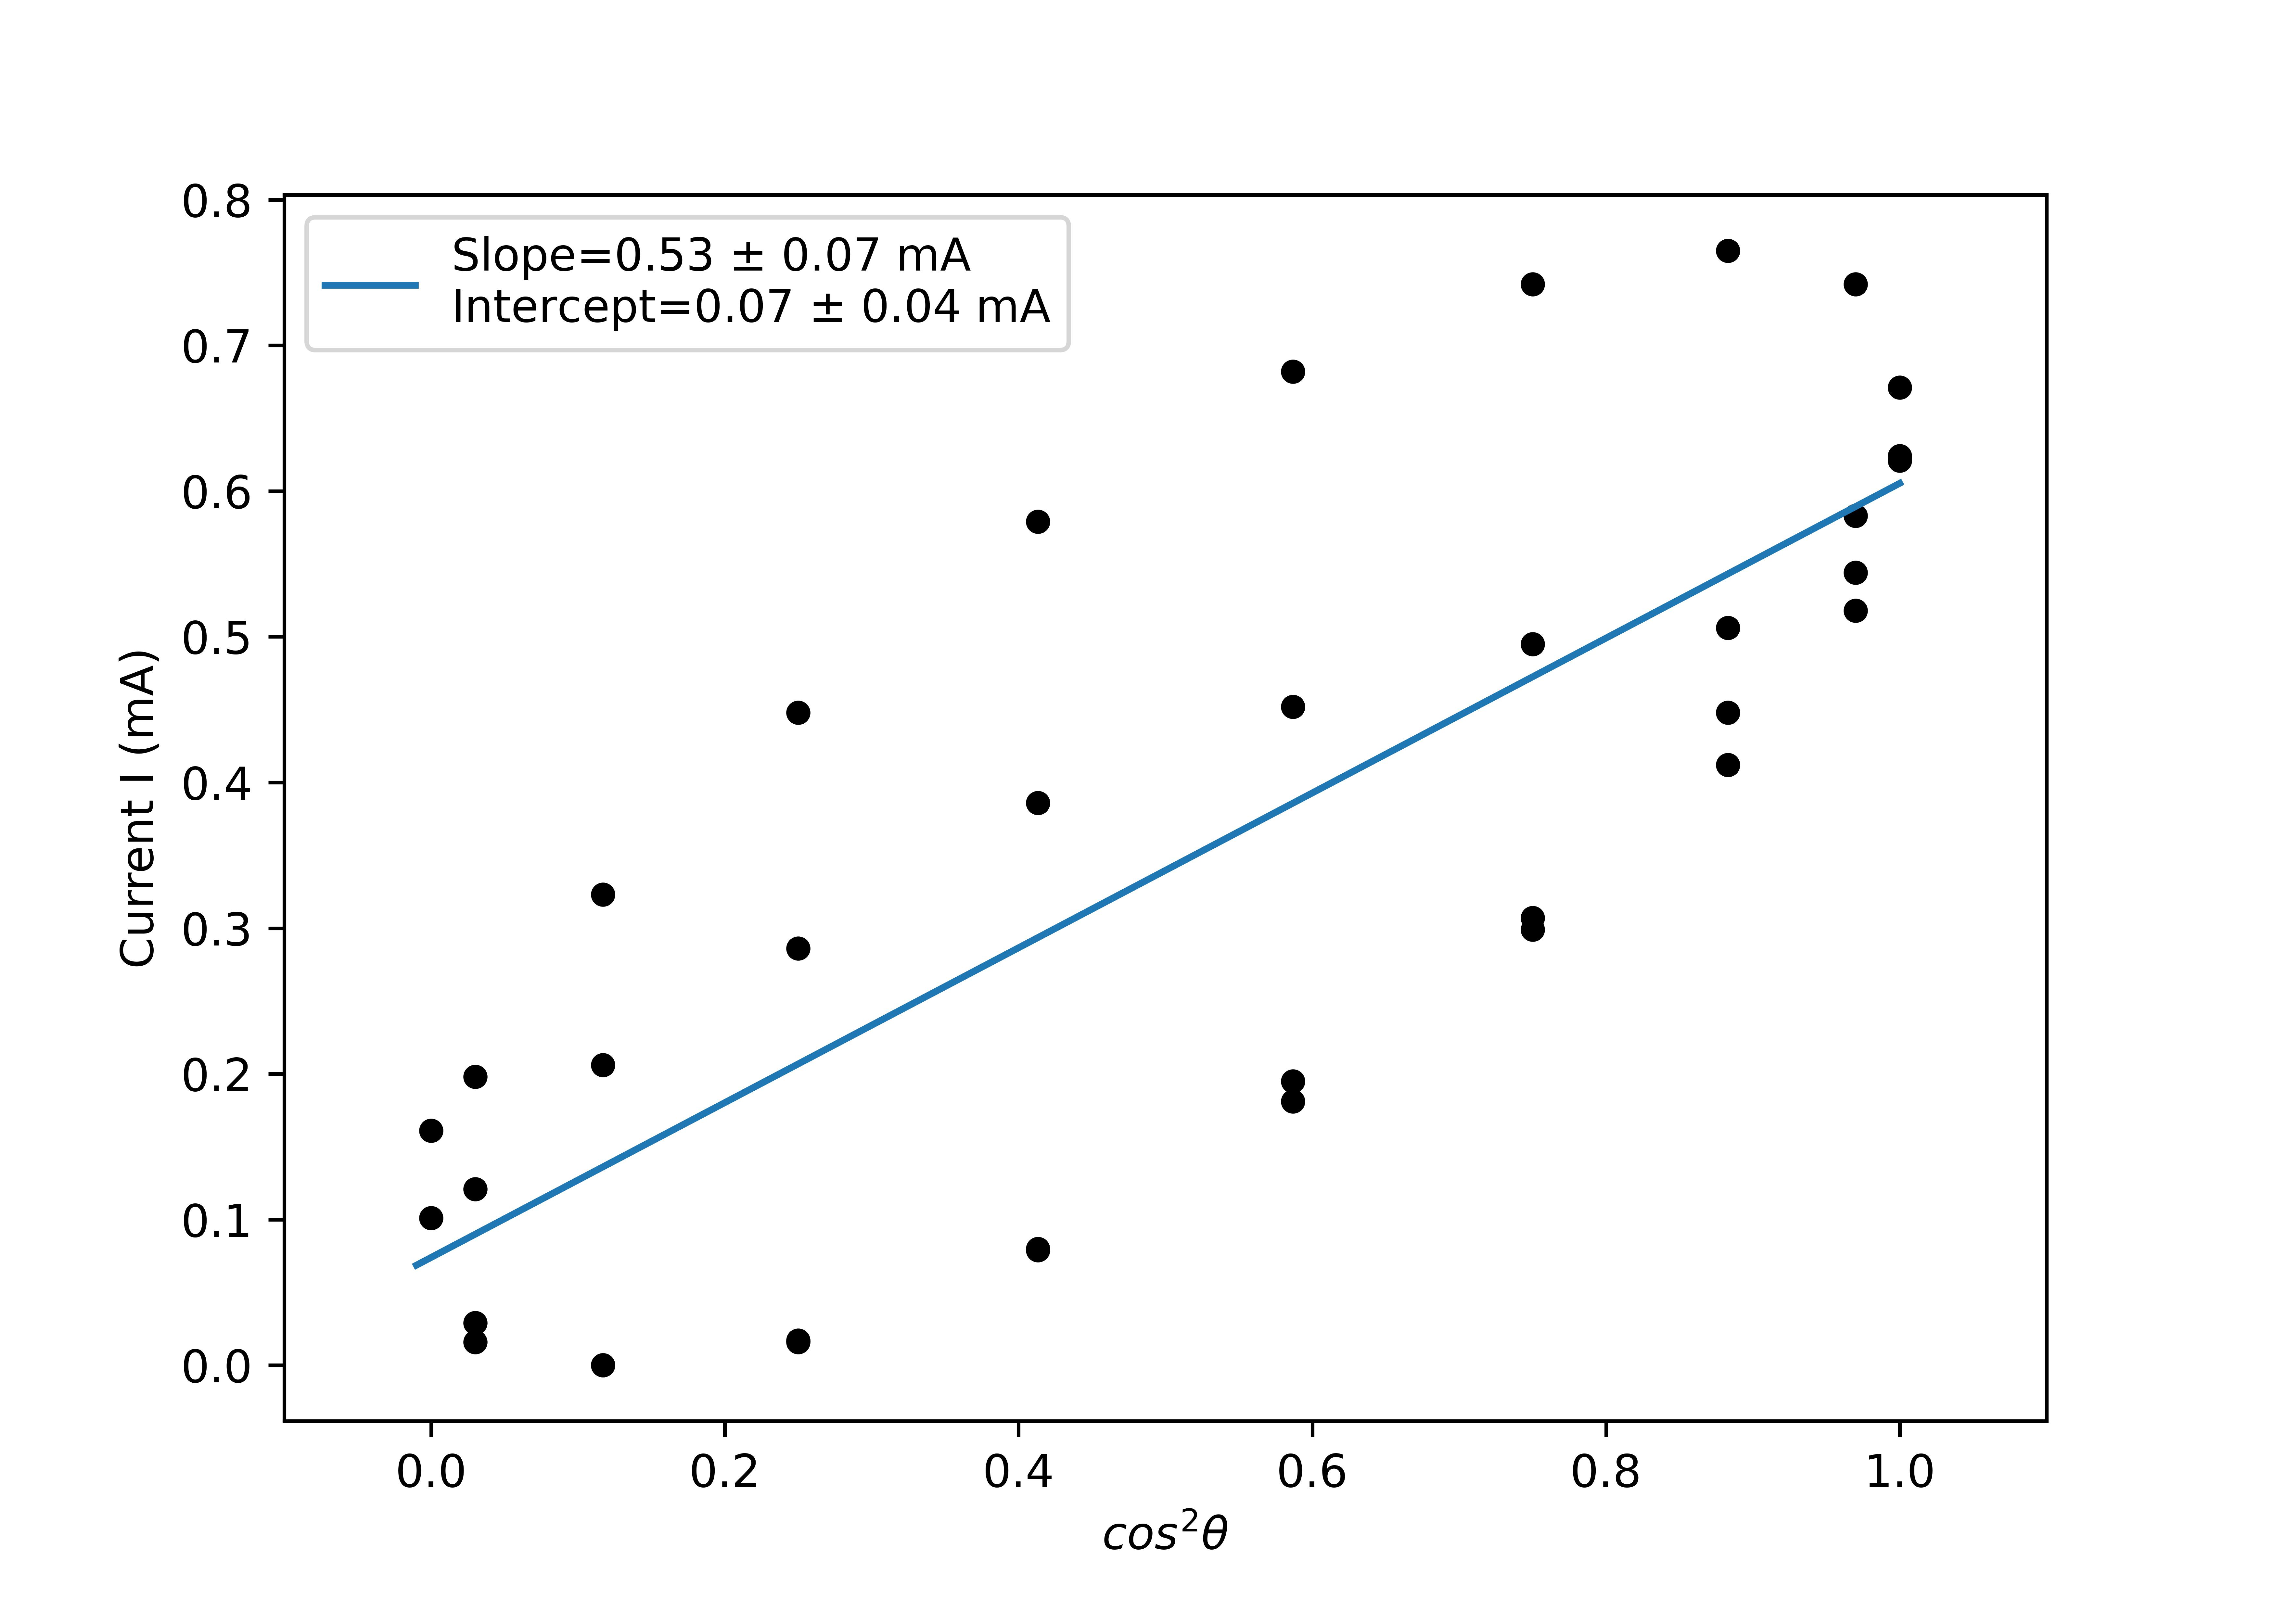
\includegraphics[width=9cm,height=8cm]{5} 
	\caption{A linear fit for the plot of current versus cosine squared of relative angle between polariser and analyser }
	\label{5}
\end{figure}

\begin{figure}[H] %  figure placement: here, top, bottom, or page
	\centering
	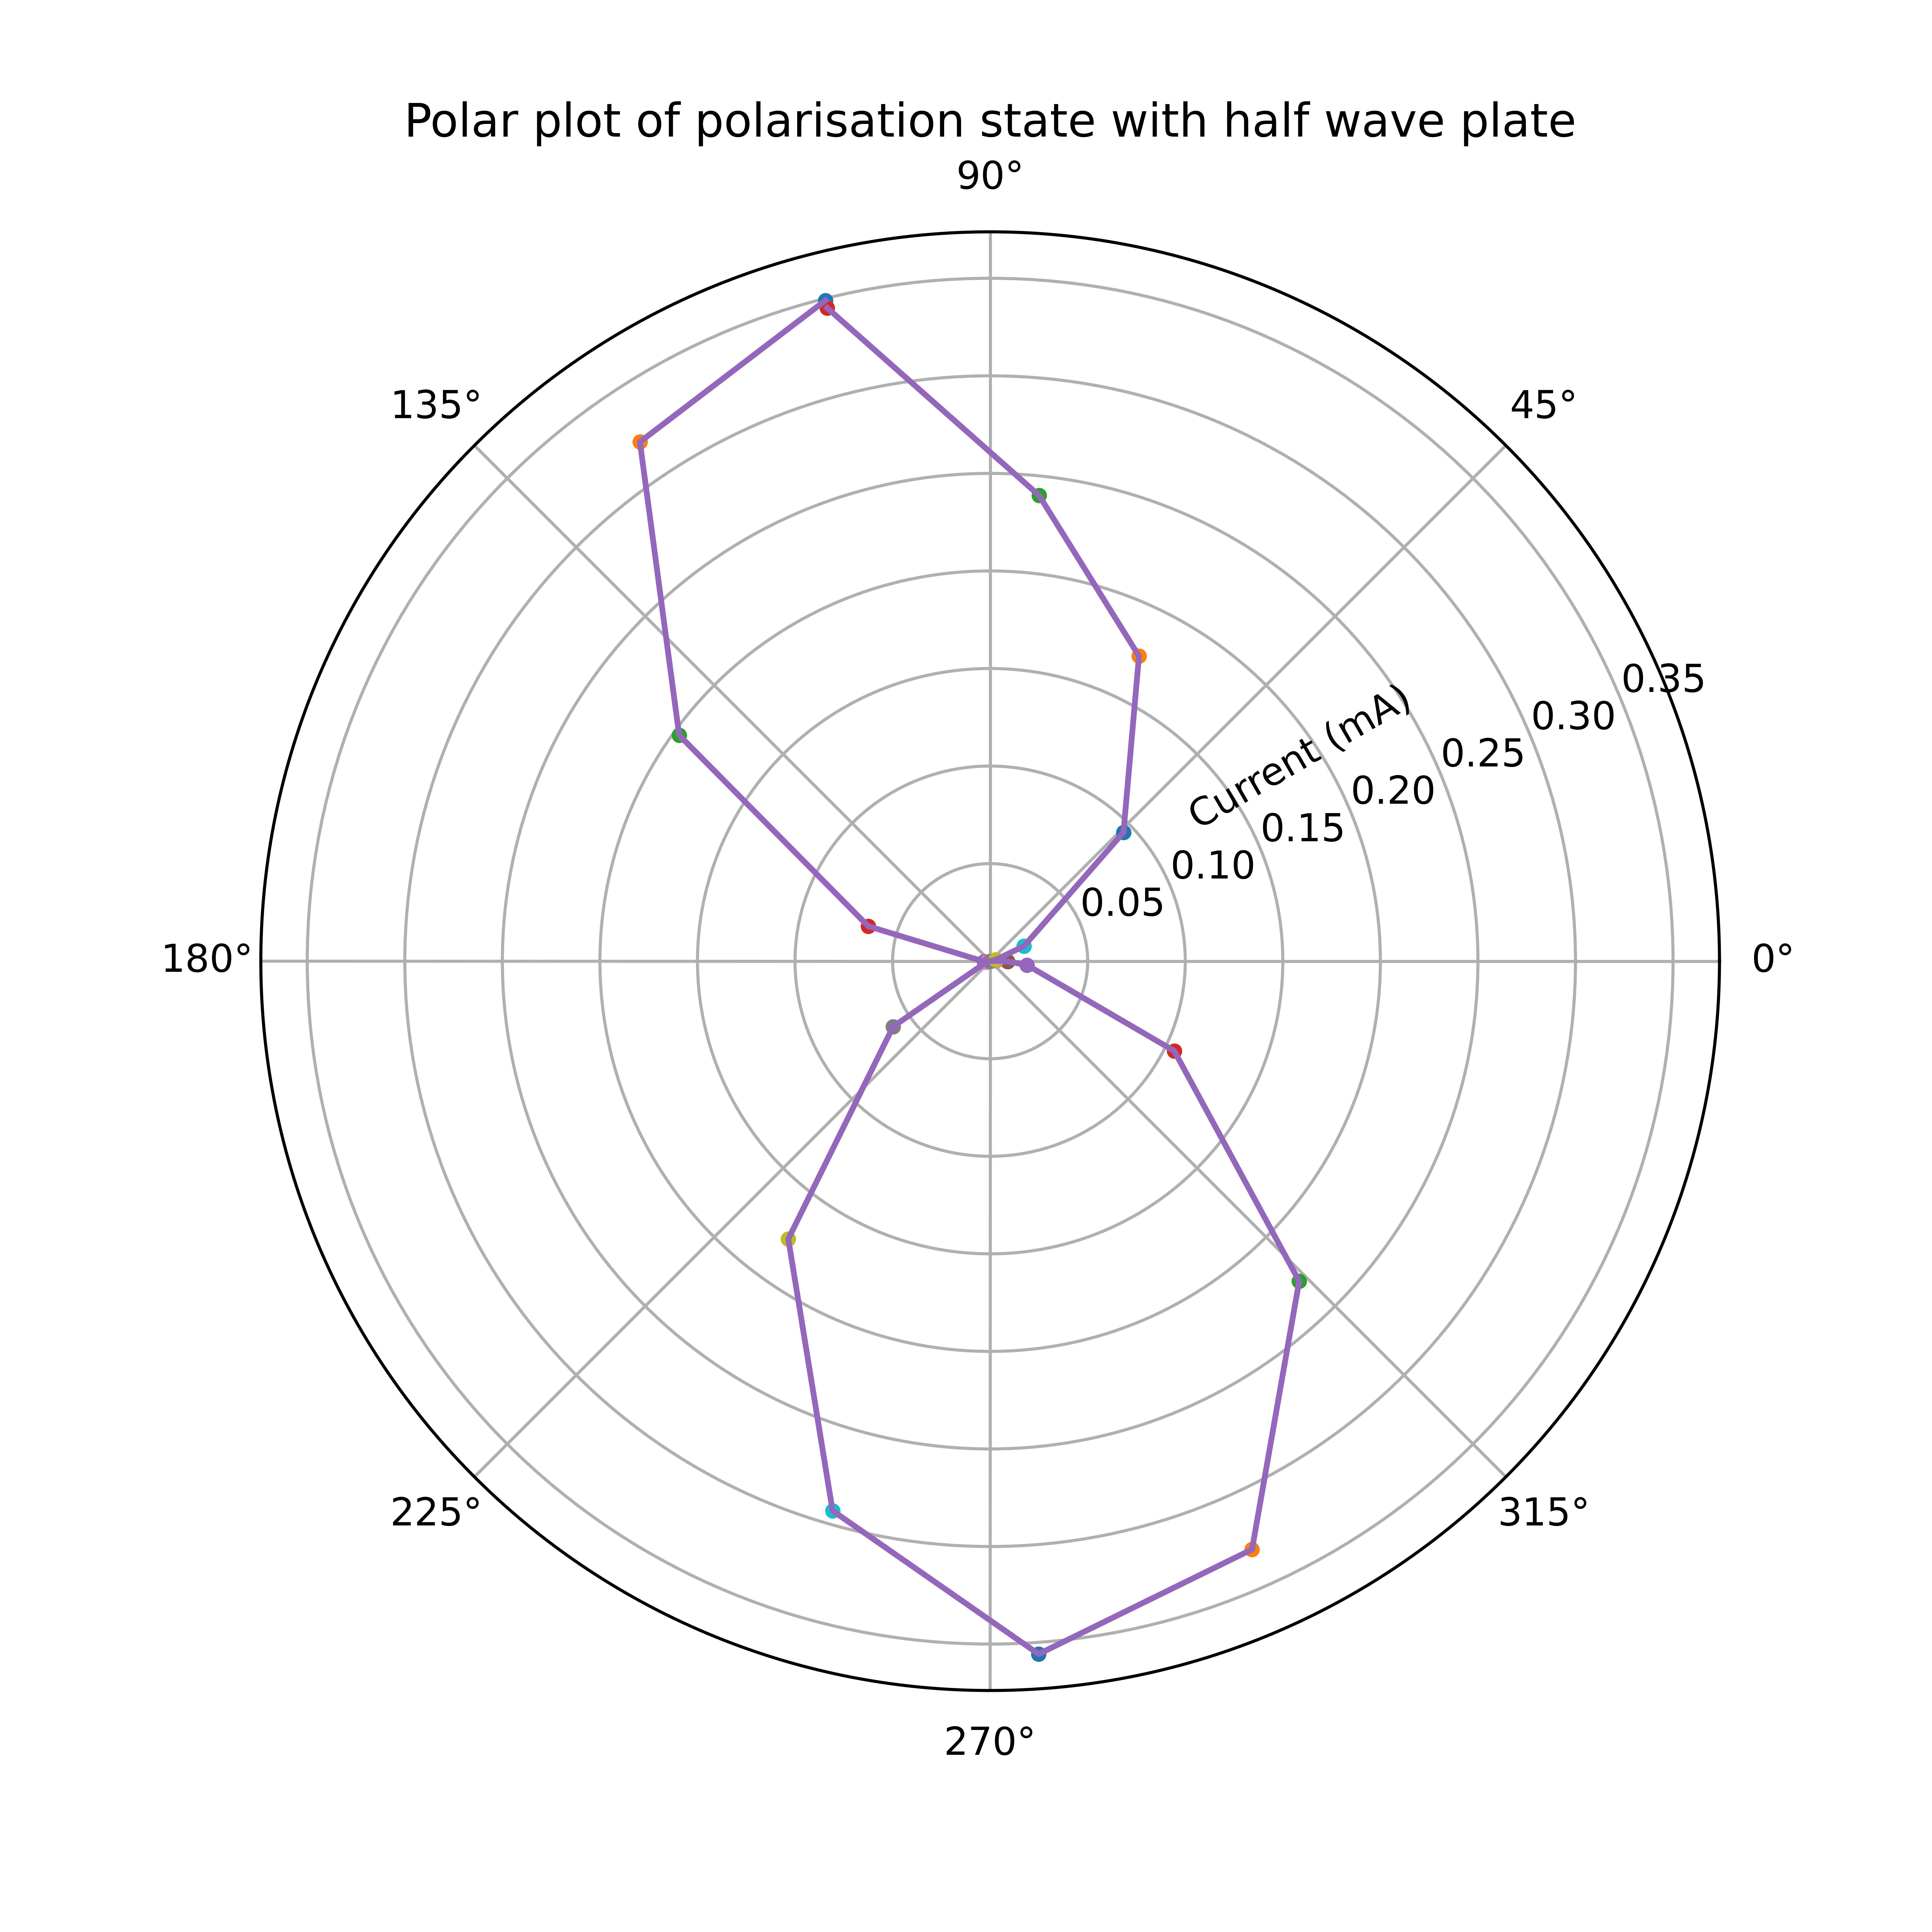
\includegraphics[width=7cm,height=7cm]{6} 
	\caption{Polar plot of linear polarisation of light with half wave plate inserted between polariser and analyser. }
	\label{6}
\end{figure}

\begin{figure}[H] %  figure placement: here, top, bottom, or page
	\centering
	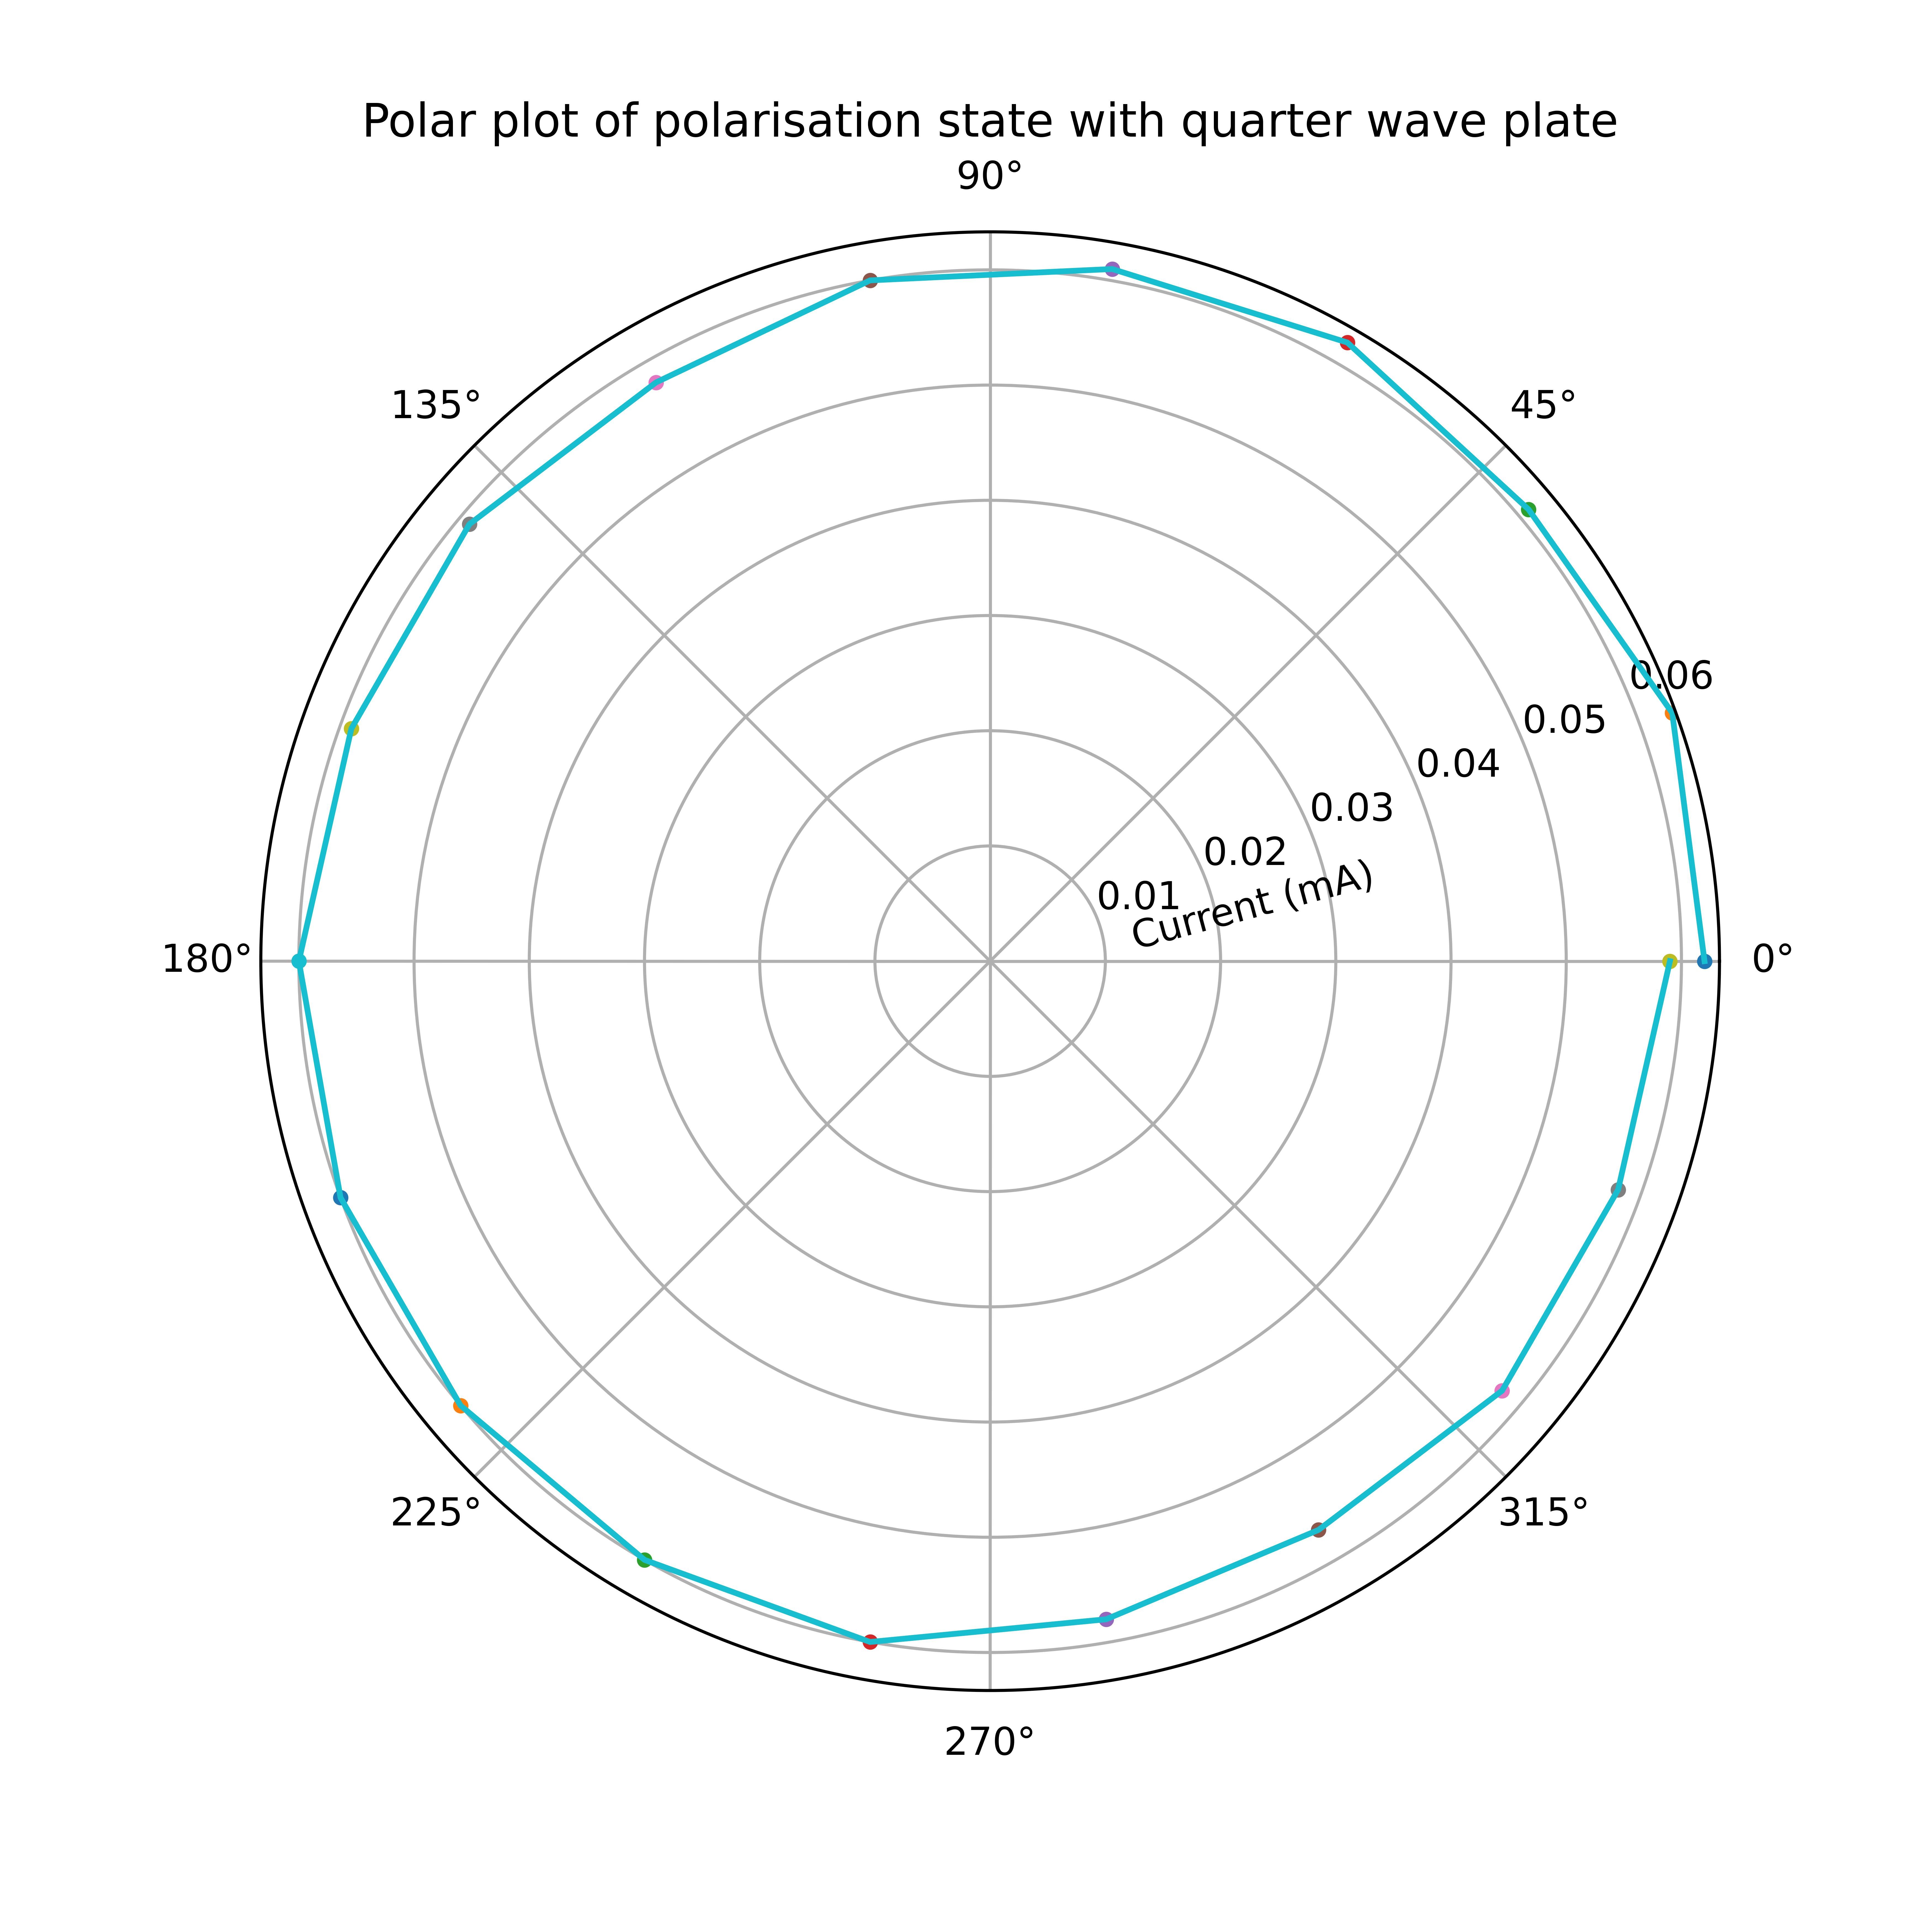
\includegraphics[width=7cm,height=7cm]{7} 
	\caption{Polar plot of linear polarisation of light with quarter wave plate inserted between polariser and analyser. }
	\label{7}
\end{figure}


We observe that the polariser and analyser when aligned with the same optical axis, the light is linearly polarised along their axis, by noting that the current is maximum when they are aligned. As we rotate it over the course of 2$\pi$, we obtain  maxima  minima. The polar plot is obtained with two petals in two hemispheres but due to heating of the photo-detector there's a slight off value to the current. If we plot the cosine square of relative angle between polariser and analyser versus photo current, we get a linear fit verifying the Malus's law. Again the off values are due to malfunctioning of photo-detector.

When we introduce the half wave plate with the orientation of plate at $45^{\circ}$, the linear polarisation shifts phase by $90^{\circ}$. It is evident by comparison of two polar plots Figure (5) and Figure (7), that the petals in plot shifts by $\pi/2$. Therefore, we can change the direction of linear polarisation to desired direction by using half wave plate. In case of quarter wave plate the current is almost constant giving circularly polarised light with the orientation of quarter wave plate at $45^{\circ}$ with the optical axis. We have obtained good circular polarisation state since, it was performed in different setup on another day, relatively better than the previous setup. 

\section{Conclusion}
In this experiment we have successfully analysed linearly polarised light by using polariser and analyser on the same optical axis, then the variation in transmitted light from analyser is directly proportional to cosine squared of angle of analyser relative to polariser axis, which satisfies Malus's law giving linear fit between $cos^2{\theta}$ and current. We also found that the half wave plate rotates the linearly polarised by 2$\theta$ if it is oriented by $\theta$ with respect to optical axis. Also, we saw that we can convert linearly polarised light into circularly polarised light by orienting quarter wave plate in $45^{\circ}$ with respect to optical axis, else we get elliptically polarised light. We studied that such birefringent materials delays and shifts the direction of polarisations. The stability and error in the experiment is reduced by using good detectors which gives stable current output. Also, it is important to block unwanted light during the experiment.

Polarisation  has wide applications such as use in spectroscopy, determining optical property of chemical compounds, sunglasses etc. Radar also uses polarisation technique.
The lenses in 3D glass are different one allows only left circular polarised light and other right circular polarised light, giving 3D image to our eyes. 
 
\section{References}
\begin{enumerate}
\item{\url{https://www.niser.ac.in/sps/sites/default/files/basic_page/Study%20of%20polarization%20of%20light.pdf}}
\item {\url{https://tikz.net/alex/polarizer-analyzer.png}}
\item {\url{https://en.wikipedia.org/wiki/Waveplate#Half-wave_plate}}
\item {\url{https://www.britannica.com/science/circular-polarization}}
\end{enumerate}
\end{document}